% A LaTeX template for MSc Thesis submissions to 
% Politecnico di Milano (PoliMi) - School of Industrial and Information Engineering
%
% S. Bonetti, A. Gruttadauria, G. Mescolini, A. Zingaro
% e-mail: template-tesi-ingind@polimi.it
%
% Last Revision: October 2021
%
% Copyright 2021 Politecnico di Milano, Italy. NC-BY

\documentclass{Configuration_Files/PoliMi3i_thesis}

%------------------------------------------------------------------------------
%	REQUIRED PACKAGES AND  CONFIGURATIONS
%------------------------------------------------------------------------------

% CONFIGURATIONS
\usepackage{parskip} % For paragraph layout
\usepackage{setspace} % For using single or double spacing
\usepackage{emptypage} % To insert empty pages
\usepackage{multicol} % To write in multiple columns (executive summary)
\setlength\columnsep{15pt} % Column separation in executive summary
\setlength\parindent{0pt} % Indentation
\raggedbottom  

% PACKAGES FOR TITLES
\usepackage{titlesec}
% \titlespacing{\section}{left spacing}{before spacing}{after spacing}
\titlespacing{\section}{0pt}{3.3ex}{2ex}
\titlespacing{\subsection}{0pt}{3.3ex}{1.65ex}
\titlespacing{\subsubsection}{0pt}{3.3ex}{1ex}
\usepackage{color}

% PACKAGES FOR LANGUAGE AND FONT
\usepackage[english]{babel} % The document is in English  
\usepackage[utf8]{inputenc} % UTF8 encoding
\usepackage[T1]{fontenc} % Font encoding
\usepackage[11pt]{moresize} % Big fonts

% PACKAGES FOR IMAGES
\usepackage{graphicx}
\usepackage{transparent} % Enables transparent images
\usepackage{eso-pic} % For the background picture on the title page
\usepackage{subfig} % Numbered and caption subfigures using \subfloat.
\usepackage{tikz} % A package for high-quality hand-made figures.
\usetikzlibrary{}
\graphicspath{{./Images/}} % Directory of the images
\usepackage{caption} % Coloured captions
\usepackage{xcolor} % Coloured captions
\usepackage{amsthm,thmtools,xcolor} % Coloured "Theorem"
\usepackage{float}

% STANDARD MATH PACKAGES
\usepackage{amsmath}
\usepackage{amsthm}
\usepackage{amssymb}
\usepackage{amsfonts}
\usepackage{bm}
\usepackage[overload]{empheq} % For braced-style systems of equations.
\usepackage{fix-cm} % To override original LaTeX restrictions on sizes

% PACKAGES FOR TABLES
\usepackage{tabularx}
\usepackage{longtable} % Tables that can span several pages
\usepackage{colortbl}

% PACKAGES FOR ALGORITHMS (PSEUDO-CODE)
\usepackage{algorithm}
\usepackage{algorithmic}

% PACKAGES FOR REFERENCES & BIBLIOGRAPHY
\usepackage[colorlinks=true,linkcolor=black,anchorcolor=black,citecolor=black,filecolor=black,menucolor=black,runcolor=black,urlcolor=black]{hyperref} % Adds clickable links at references
\usepackage{cleveref}
\usepackage[square, numbers, sort&compress]{natbib} % Square brackets, citing references with numbers, citations sorted by appearance in the text and compressed
\bibliographystyle{abbrvnat} % You may use a different style adapted to your field

% OTHER PACKAGES
\usepackage{pdfpages} % To include a pdf file
\usepackage{afterpage}
\usepackage{lipsum} % DUMMY PACKAGE
\usepackage{fancyhdr} % For the headers
\fancyhf{}

% Input of configuration file. Do not change config.tex file unless you really know what you are doing. 
% Define blue color typical of polimi
\definecolor{bluepoli}{cmyk}{0.4,0.1,0,0.4}

% Custom theorem environments
\declaretheoremstyle[
  headfont=\color{bluepoli}\normalfont\bfseries,
  bodyfont=\color{black}\normalfont\itshape,
]{colored}

% Set-up caption colors
\captionsetup[figure]{labelfont={color=bluepoli}} % Set colour of the captions
\captionsetup[table]{labelfont={color=bluepoli}} % Set colour of the captions
\captionsetup[algorithm]{labelfont={color=bluepoli}} % Set colour of the captions

\theoremstyle{colored}
\newtheorem{theorem}{Theorem}[chapter]
\newtheorem{proposition}{Proposition}[chapter]

% Enhances the features of the standard "table" and "tabular" environments.
\newcommand\T{\rule{0pt}{2.6ex}}
\newcommand\B{\rule[-1.2ex]{0pt}{0pt}}

% Pseudo-code algorithm descriptions.
\newcounter{algsubstate}
\renewcommand{\thealgsubstate}{\alph{algsubstate}}
\newenvironment{algsubstates}
  {\setcounter{algsubstate}{0}%
   \renewcommand{\STATE}{%
     \stepcounter{algsubstate}%
     \Statex {\small\thealgsubstate:}\space}}
  {}

% New font size
\newcommand\numfontsize{\@setfontsize\Huge{200}{60}}

% Title format: chapter
\titleformat{\chapter}[hang]{
\fontsize{50}{20}\selectfont\bfseries\filright}{\textcolor{bluepoli} \thechapter\hsp\hspace{2mm}\textcolor{bluepoli}{|   }\hsp}{0pt}{\huge\bfseries \textcolor{bluepoli}
}

% Title format: section
\titleformat{\section}
{\color{bluepoli}\normalfont\Large\bfseries}
{\color{bluepoli}\thesection.}{1em}{}

% Title format: subsection
\titleformat{\subsection}
{\color{bluepoli}\normalfont\large\bfseries}
{\color{bluepoli}\thesubsection.}{1em}{}

% Title format: subsubsection
\titleformat{\subsubsection}
{\color{bluepoli}\normalfont\large\bfseries}
{\color{bluepoli}\thesubsubsection.}{1em}{}

% Shortening for setting no horizontal-spacing
\newcommand{\hsp}{\hspace{0pt}}

\makeatletter
% Renewcommand: cleardoublepage including the background pic
\renewcommand*\cleardoublepage{%
  \clearpage\if@twoside\ifodd\c@page\else
  \null
  \AddToShipoutPicture*{\BackgroundPic}
  \thispagestyle{empty}%
  \newpage
  \if@twocolumn\hbox{}\newpage\fi\fi\fi}
\makeatother

%For correctly numbering algorithms
\numberwithin{algorithm}{chapter}

%----------------------------------------------------------------------------
%	NEW COMMANDS DEFINED
%----------------------------------------------------------------------------

% EXAMPLES OF NEW COMMANDS
\newcommand{\bea}{\begin{eqnarray}} % Shortcut for equation arrays
\newcommand{\eea}{\end{eqnarray}}
\newcommand{\e}[1]{\times 10^{#1}}  % Powers of 10 notation

%----------------------------------------------------------------------------
%	ADD YOUR PACKAGES (be careful of package interaction)
%----------------------------------------------------------------------------

%----------------------------------------------------------------------------
%	ADD YOUR DEFINITIONS AND COMMANDS (be careful of existing commands)
%----------------------------------------------------------------------------

%----------------------------------------------------------------------------
%	BEGIN OF YOUR DOCUMENT
%----------------------------------------------------------------------------

\begin{document}

\fancypagestyle{plain}{%
\fancyhf{} % Clear all header and footer fields
\fancyhead[RO,RE]{\thepage} %RO=right odd, RE=right even
\renewcommand{\headrulewidth}{0pt}
\renewcommand{\footrulewidth}{0pt}}

%----------------------------------------------------------------------------
%	TITLE PAGE
%----------------------------------------------------------------------------

\pagestyle{empty} % No page numbers
\frontmatter % Use roman page numbering style (i, ii, iii, iv...) for the preamble pages

\puttitle{
	title=WIP Title: Dynamic resource allocation in the cloud for compute heavy tasks in a containerized environment,
	name=Elia Ravella,
	course=Computer Science and Engineering,
	ID  = 967243,
	advisor= Prof. Raffaela Mirandola,
	coadvisor={Name Surname, Name Surname},
	academicyear={2021-22},
} % These info will be put into your Title page 

%----------------------------------------------------------------------------
%	PREAMBLE PAGES: ABSTRACT (inglese e italiano), EXECUTIVE SUMMARY
%----------------------------------------------------------------------------
\startpreamble
\setcounter{page}{1} % Set page counter to 1

% ABSTRACT IN ENGLISH
\chapter*{Abstract} 
\textbf{Keywords:} Cloud, Containers, Dynamic infrastructure

%----------------------------------------------------------------------------
%	LIST OF CONTENTS/FIGURES/TABLES/SYMBOLS
%----------------------------------------------------------------------------

% TABLE OF CONTENTS
\thispagestyle{empty}
\tableofcontents % Table of contents 

\addtocontents{toc}{\vspace{2em}} % Add a gap in the Contents, for aesthetics
\mainmatter % Begin numeric (1,2,3...) page numbering
	\chapter{The Problem and the Current Available Solutions}
		\section{Introduction}
		\label{se:introduction}
    
    \section{The Problem}
		\label{se:problem}
    Scalability is one of the key design point that must be taken into consideration when developing a software. If a system cannot scale in power when the userbase or the load requested changes it slows down, making the response times growing for each request and compromising the overall performance of the application. The most intuitive approach to scalability, which is also the most common in cloud environments, is horizontal replication. With horizontal replication I mean (throughout all this thesis) the addition of identical software modules alongside the already existing ones to share the load; to do so, different incoming requests are routed to different modules when they arrive. The replicas being identical (and usually stateless) ensure that each request is carried out in the same way. The policies for deploying replicas can be either static or dynamic (based on the predicted load during the day or measuring the real time traffic incoming, for example).\\

This approach has seen a wide adoption in the industry and is the \textit{de facto} standard to tackle scalability problems, especially in web environments. The horizontal replication approach gives applications the flexibility they need in reacting to the load that is applied, and is especially effective when the application is divided in submodules that can be individually scaled.\\

What happens when the requests that an application must serve change also in nature, and not only in volume? Horizontal replication works well when the load is mostly uniform (and for the majority of web applications, it is) and can be analyzed in a one dimensional fashion as "the number of requests". When requests set in motion heavy computational pipelines, as image processing or complex mathematical problems, but the interface they are served is shared with all the other \textit{light} requests\footnote{this is not an impossible scenario: what a REST API exposes are a list of "light" HTTP requests that can trigger all kind of operations on the server they are executed on} then a single request can weight, in terms of resources it needs to be carried out, very differently from the others. In this scenario, horizontal replication is harder to put in place effectively: if requests weight differently it is not possible to just share them equally among replicated servers\footnote{here \textit{servers} is used to describe logical backend modules, not physical machines} because in some cases a server will receive a much more higher share of heavy requests and be stuck executing them while other servers will be idling because they received only light requests. Horizontal replication, as it is implemented now, cannot face efficently this scenario. The proposed solution uses dedicated ephemeral workers to execute \textit{heavy} requests, and organises and schedules them with a ticketing middleware. 

	
		\section{Containerized Environment and High Performance Computing}
		\label{se:containerHPC}
    %% Section: Container and HPC
\paragraph{Containerization}
  Virtualization is "the act of creating a virtual (rather than actual) version of something at the same abstraction level, including virtual computer hardware platforms, storage devices, and computer network resources"\cite{wiki:virtualization}. In cloud environments virtualization is the most used tool to provide isolated services, as compute capabilities, storage capabilities or networking. There are different kinds of virtualization, depending on the layer virtualized: some solutions just virtualize the hardware and let the user install a full fledged OS over it, other virtualizes all the technological stack from the hardware to the OS level, leaving to the user (in most of the cases, a developer) only the problem of developing the application s/he wants to ship, without the need to care about hardware limitations or operative systems settings.\\
  
  One of the most used virtualization technique in the industry is containerization: when a software is said to be \textit{containerized} it is packaged in a format that encapsulates also all its dependencies, configuration files and variables and OS settings. This package, the container, must be run through a container engine (or equivalent operative system module) which provide the communication with the underlying software and OS to execute the software. Famous container engines are Docker, Podman, chroot or rkt, but containers were originally supported by Linux OS in form of "special processes" (the so called LXC containers). Containerized applications have several benefits over classic deployed ones:
  \begin{itemize}
    \item They do not rely on the machine or OS they are running, just the engine
    \item If the container has been built correctly, the configuration of the application is already done
    \item Packaging all their dependencies makes them independent from the other application installed on the system: two containerized applications running on the same engine could be using the same library but at different (and even incompatible) versions
    \item The container acts also as an isolation mechanism, that keeps the application from interacting with other systems: this improves the security of the container applications
  \end{itemize}
  
  If an application is containerized, moreover, it is very easy to deploy several instances of the same application working at the same time: this kind of deployments improve scalability and reliability of the application.\\

\paragraph{High Performance Computing}
  With "high performance computing" is usually addressed the field in computer science that studies computational heavy problems and develops solutions to solve them via techniques as extreme parallelism, clusterization and high performance networking. In the early stages of this project we focused also on HPC in order to understand if a virtualization approach as the containers one is suitable for such kind of tasks. The problem was the additional layer of virtualization added by the container engine: since most of the times HPC software relies heavily on low-level procedure calls, the additional virtualized layer could degrade too much the performance. However, as stated in the paper "Exploring the support for high performance applications in the container runtime environment"\cite{containershpc2} (which original aim was to compare native performance with containerized ones) the optimization of engines is reaching a level that can offer near-native performance for HPC-like loads, at least in not-extreme scenarios.

		
		\section{State of the Industry}
		\label{se:stateoftheart}
    There are several solutions available on the market that provides flexible infrastructure management and are built to automate the management of the infrastructure of an application. These systems can be seen as schedulers (so software components that organize when a task is executed and on which resources) with some additional features as the capability of actually \textit{allocate} the resources needed or the automated management of the interfaces between resources and components.

\subsection{SLURM}
\label{sse:slurm}
  SLURM is "an open source, fault-tolerant, and highly scalable cluster management and job scheduling system for large and small Linux clusters"\cite{slurm}. It aims to organize and schedule tasks on multiple nodes; these tasks can also be defined as OCI-compliant containers. SLURM was crated to be executed on supercomputers or clusters of computers; in fact, SLURM focuses on communication between daemons and tasks through message passing framework as MPI and queue-managed resource access. Even if it can integrate containerized workloads, it is not suited to be deployed in a cloud environment rather than a computation center.

\subsection{Shifter}
\label{sse:shifter}
  Shifter is a simple scheduler which aims to utilize the container format in an HPC environment. It allows the user to specify the load in a docker image, then Shifter automates the conversion of that image to an HPC format and the scheduling of such task. Shifter is \textit{not} an extension of Docker or the Docker engine, nor aims to automate the infrastructure, instead it just provides an additional interface (which is container compatible) to an already existing HPC platform.

\subsection{Kubernetes}
\label{sse:kubernetes}
  Kubernetes (often called "k8s") is a container orchestration system, and is the \textit{de facto} standard for container orchestration. It provides an all-in-one system to manage containerized applications:
  \begin{itemize}
    \item It provides an abstraction over the container level (the Pod) that is used to define the service provided rather than the container itself
    \item It includes different ways to persist data and state across containers; this gives a kubernetes cluster the capability to hold an entire application, from data layer to presentation layer
    \item Kubernetes clusters embeds security and access control by enforcing the already existing isolation features of a containerized environment and by providing a set of tools that easily control the access to the cluster itself (the Ingress controllers)
    \item It allows developers to define the redundancy for every single service defined, so to set an "horizontal scaling width" beforehand to handle faults and heavy loads
  \end{itemize}
  Kubernetes has been designed for applications that are designed as microservices, and it provides the tooling for administrate single services, replication, and scaling in such an environment. As already stated in (\ref{se:problem}) the level of abstraction provided by kubernetes is efficent when horizontal scaling must be automated, but also removes some of the controllability of a containerized system. Moreover, resource management within kubernetes deployment in the cloud is very difficult: all the needed resources must be available at any time so that kubernetes can manage them, and this implies reserving significant amounts of resources for a prolonged period of time; in a cloud deployed application this renders the cost of application maintenance too high. 

\subsection{Serverless Approach}
\label{sse:serverless}

			
		
	\chapter{Design and Testing Phase}
	\label{ch:designandtesting}

		\section{MapNCloud Original Architecture}
		\label{se:originalarchitecture}
    This thesis project extends and develops the original Distributed Software Development project, which have been created during the first semester of the 2021 / 2022 academic year. The original project aim was to create a system which could offer photogrammetry services, so the rendering of a tridimensional model from a set of images of the subject, leveraging the container technology to encapsulate the rendering engine. In this section we describe the original architecture of that system and in the next ones we will explain how that architecture has been redesigned, adapted and extended in this thesis project. 

\subsection{System Design}
\label{sse:originalsystemdesign}
  The MapNCloud project was designed as a "three plus one" tiers application:
  \begin{itemize}
    \item a \textbf{presentation layer} or front end, which has been developed as a web site and offers a graphical interface to the system
    \item a \textbf{business layer} or back end, which embodies all the business logic of the application
    \item a \textbf{data layer}, the database which persists the data needed by the application
    \item a \textbf{computation layer}, which is a separated back end module that is tasked with the most computational heavy routines (as the photogrammetry pipelines)
  \end{itemize}
  Another module is present in the application, and it is the ticketing service. It is not considered a whole tier, in fact its only job is to manage the queues of tasks that the backend generates, and let the computational layer components access them in the right order with the right schedule.
  \begin{figure}[H]
    \centering
    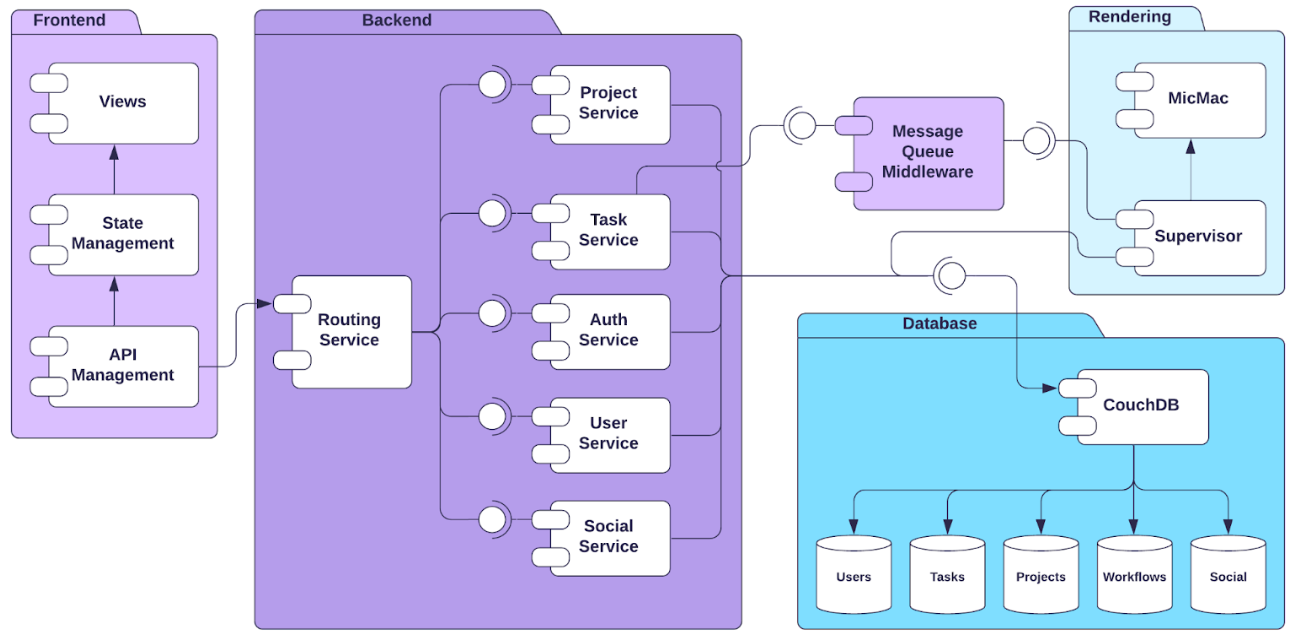
\includegraphics[width = \textwidth]{../Images/MNCOriginal.png}
    \caption{Original MapNCloud component diagram, with internal modules detailed.}
  \end{figure}

  \subsubsection{Front End}
  \label{ssse:originalfrontend}
    The presentation layer of the application was developed as a web application; this exposes a graphical user interface for the services offered by the system. It is a JavaScript application (developed with the VueJS framework) which interacts with the backend via HTTP calls; this allows it to be considered, by the cloud provider, a static web application, which is easy to deploy and has a low resources demand.\\
    The front end architecture follows the Model View ViewModel pattern, which separates the actual GUI elements from the logic of the user experience in View and ViewModel respectively, and lets the ViewModel reflect the changes on the Model; this is a common pattern to adopt as it provides a clear organization of functionalities and responsibilities among the internal software submodules.\\
    The front end is deployed as a static web app in the cloud provider web hosting dedicated service. It is directly built and made available from the code repository (through a CI/CD pipeline) reacting at every code change on a specific branch. The cloud provider also takes care of the SSL certificates (to ensure crypted communication) and the global availability through content delivery networks.\\
    The front end module is the one that is the least affected by this thesis work; it is only extended to include an administration section.

  \subsubsection{Back End}
  \label{ssse:originalbackend}
    The backend module is composed of two main software modules, which are distinct applications:
    \begin{itemize}
      \item the actual MapNCloud backend, a TypeScript application that exposes a REST API with all the functionalities of the application. This module is packaged as a Docker container; in this scenario, the possibility to bundle together code, configuration files and additional resources in a single Docker image makes deployment faster and easier, also providing all the isolation properties offered by the containers alone.
      \item a queue managing system, which acts as the ticketing system for the tasks issued to the computation layer. This is a RabbitMQ (a popular open source queue management system) instance, communicating via AMQP\cite{AMQP} with the other modules. The choice to separate these modules was taken to ensure the reliability of the whole system, and to enhance the maintainability of it (RabbitMQ offers out of the box monitoring services, which help to diagnose and follow the instance execution. These were to be reimplemented from scratch if the queuing module were implemented together with the application). This module is also deployed as a Docker container, but in this case the choice was made to reduce the amount of infrastructure needed for the application: the alternatives were deploying a single container group with RabbitMQ and the computational layer together or provisioning a whole virtual machine just for installing a whole instance of RabbitMQ.
    \end{itemize}
    The backend is the module that is most affected by this thesis work: in the next section the major changes will be analyzed, which affect the internal organization of components, the use of the tools offered by RabbitMQ and the positioning of the module in the overall architecture.
  
  \subsubsection{Data Layer}
  \label{ssse:originaldatalayer}
    The Data Layer is the component of the application that persists the data generated by the system, organizes it and make it available to the backend itself to distribute it. It is in charge of storing, as a example, the source files for the photogrammetry processes, the output 3D models, and all the data (stored as hierarchical text data) which describe the users, the projects and the tasks generated by the users themselves.\\
    The DB choice was CouchDB, a non relational database produced by Apache and is written in the same highly parallel technology of RabbitMQ; this also simplifies the deployment of clusters instead of single instances. The choice of non-relational was made to help in the earlier stage of development, where the flexibility of such an approach helped us in prototyping. As per the queuing system, this module is packaged, configured and deployed as Docker container.
    
  \subsubsection{Computation Later}
  \label{ssse:originalcomputationlayer}
    The "fourth layer" is the one that carries out the heavy computational tasks issued by the backend. It is composed by several independent \textit{workers}, which are simply containers, that are separated from the backend to ensure that it does not get stuck on a single request. These containers' internal architecture is rather simple: the chosen engine (during the original development MicMac) is wrapped in an external TypeScript application which divides the various phases of the pipeline in "Stages" and so extends the capabilities of the of the original engine: these Stages can be configured by the user (they are part of the data model memorized in the DB, in fact).\\
    The computational backend has to interact with the queuing system to retrieve the tasks and with the DB to get the resources and output the computed results. This "circular" dependency between backend modules is highlighted here because will be the cause of some major change in the backend architecture. The container technology here is leveraged to ensure a fast spin-up time for a worker (which will be significantly longer for a VM, considering also the complex installation process of such engines) and the reusability of the images, which allows for a fast resize and scale of this layer of the architecture.


		\section{Problems Addressed}
		\label{se:problemsaddressed}
    The original application was packaged and deployed as a self-hostable stack: a group of containerized applications all in the same configuration files, which used docker-compose as the orchestration tool. This simple deployment solution was suited for the demo required for the original project, but the really limited support cloud providers offer to the docker-compose tool\footnote{at the moment of writing, several cloud providers has early-development stage support for docker compose, moreover further limited to only a few container-oriented services.} and the future necessity to dynamically scale the backend modules rendered this approach non suitable. In this section we will address the major problems the architecture had in the first place, how these were faced and which decisions were taken to overcome them.

\subsection{Scalability}
  The MapNCloud system was designed to ensure a detachment between the "business logic" backend and the "computational" backend, in order to ensure that that the full application does not get stuck on a request by offloading longer tasks to a different independent module. This module (\ref{ssse:originalcomputationlayer}) is the main bottleneck of the system, and though the one we focused on to improve its overall scalability.\\
  The first approach considered was to use an automated orchestration software as Kubernetes (\ref{sse:kubernetes}) or a task scheduler as SLURM (\ref{sse:slurm}) to manage the mapping of tasks on available computational units; as explained in the respective sections, these approaches were not viable, due to either an high infrastructure cost or a poor cloud compatibility. The system was required to be able to handle different traffic paces, with different requests weights, being at the same time cost effective\footnote{which translates, in cloud environments, to deallocate unused resources}.\\
  The target solution needed to dynamically spawn workers, each one tailored to the actual traffic detected or to a forecast on traffic (based on past data or statically, using time of day as index for example). Each worker had to be spawned with a different set of resources, to better handle the traffic. As an example, if a great number of requests suddenly arrive all together, each one with an high number of input files, some resourceful workers needed to be spawned; instead, if the number of unacknowledged tasks grows steadily but slowly, a smaller\footnote{smaller in the number or size of resources allocated: number of CPUs, amount of RAM and optional GPUs} worker unit can be created to handle the accumulating tasks. This kind of reasoning \textit{must} be applied also in the other direction: especially in the cloud, systems that allocates a significant number of hardware resources are very expensive; if heavy workers (i.e. some modules with high CPU or GPU count) are idling, or the system can satisfy the incoming traffic without them, in order to be cost effective the system should be able to identify the unnecessary workers and kill them. The final design uses an automation tool provided by the cloud vendor to expose a REST interface that allows an alerting module (built in the queuing system) to notify congestion situations, and to also shape the worker spawned in terms of CPU count, GPU count and memory available.

\subsection{Cloud Provider Integration}
  The choice of the cloud provider was discussed in the first steps of the project, and after some initial performance tests Azure by Microsoft has been chosen. These simple tests were conducted to see if there was a significant difference in performance between the two vendors: the results are available in the dedicated appendix. In the choice of the cloud vendor other factors have been relevant, as the ease of integration between internal services, general support provided by the vendor itself, migration problems and developer familiarity with the tools.

\subsection{Queue Monitoring}
  The queue module is the one that is "congestion aware". The workers are designed to interact with it by dequeuing a message (which contains all the task-related information), processing the task and only when the task has been successfully executed and completed acknowledge the message to the queue. This provides a straightforward metric to both understand congestion of the queues and of the workers: the combination of unacknowledged messages and the ones entirely not delivered to clients. A majority of unacknowledged messages would suggest that the workers are underpowered, while a majority of not delivered messages would suggest that too few workers are deployed. These kind of metrics and indexes must be extracted from the queuing system in order to manage the number of workers present.\\
  Luckily, RabbitMQ embeds a monitoring tool (called Prometheus) which automatically organizes the queues data and exports them in a text format. An additional module of Prometheus, called AlertManager, handles the notifications and interacts with external services; this fits perfectly our use case, allowing us to group together various pieces of information and deliver a precise alert (which will be encapsulated in a HTTP request) that actively reshapes the backend to align to the congestion status.\\
  In the early design steps, it was considered to use a cluster of RabbitMQ instances rather than a single one, to improve on reliability and resilience. The cluster additional copies of RabbitMQ would have provided an higher failure tolerance, since the whole cluster could then withstand a failure of an instance, up to "all but one" instances failure. This option was discarded:
  \begin{itemize}
    \item Using a set of instances in place of a single one requires either to inform the other modules of the fallback options or to use a load balancer put in front of the RabbitMQ cluster to interact with it: in the former case all the backend modules would have needed an additional modification; in the latter, an additional software component should have been inserted in the architecture and configured, with the risk of degrading performance
    \item Tests were conducted to assure if a single RabbitMQ instance could withstand the load imposed by the application, in different scenarios (as single backend workers versus dynamic resizing backend workers). These tests are available in the appendix
    \item Clustering RabbitMQ nodes, although a very powerful feature of that software and surely fundamental in large distributed message oriented scenarios, requires some additional per-node configuration which would have itself complicated the deployment of the system
  \end{itemize}

\subsection{API Redesign and Organization}
  The module that mostly is impacted by this thesis' work is the backend. From the original design (\ref{ssse:originalcomputationlayer}) the module has been separated in two main components
  \begin{enumerate}
    \item the \textbf{MainBackend}: this module actually hosts the exposed Application Programming Interface the frontend utilizes. The interface exposed is very similar to the original one, the major changes residing in the data access layer\footnote{further details on the original architecture available in appendix (\ref{ap:originaldesigndoc})} which no longer interfaces directly with the database, but instead calls another API to interact with it for tasks as attachments searching and retrieving, data access (which encapsulates authentication) and uploading of resources.\\
      This piece is software is deployed as an Azure Web App exposed on the internet (which is in contrast with most of the other components of the architecture, which are deployed inside a virtual network) and is packaged as a container. This is the module that encapsulates the business logic of the application. It exposes an interface to the frontend to be utilized and interacts with the OperationalBackend to handle the data (images, models, user data) and the task management functions, as interfacing with RabbitMQ to add a task to be executed. It interacts with the other components just through REST interfaces.
    \item the \textbf{OperationalBackend}: this module is deployed as an Azure Web App also, and moreover it is assigned at the same hosting and scaling plan of the Main one (which are called Azure App Services); differently from the Main one, though, it is deployed inside a dedicated subnet of the Virtual Network used to isolate the system. This module however is additionally secured, allowing among all incoming requests only the one originating from the MainBackend to actually be processed. This has two major benefits: firstly, making sure that only requests from a "secure" origin can penetrate the virtual network and reach the OperationalBackend, and then to avoid the waste of resources to process "useless" requests.\\
      Like the Main one, this backend is packaged and deployed as a Docker container; being this the component that also initializes the database and the queue system, and so uses many different configuration and initialization files, the docker packaging mechanism is useful to keep all the app configuration organized together.\\
      This component has a variety of roles:
      \begin{itemize}
        \item it exposes a REST interface for the MainBackend that implements the basic CRUD\footnote{Create Read Update Delete} operations for the data models of the applications, acting like a "proxy" of the database
        \item the same API has a set of endpoints dedicated to the computational layer modules, the "renderini", to operate (as an example) group resources handling
        \item it interfaces with RabbitMQ via AMQP channels to add tasks for the computational layer to be executed
        \item it needs to connect to the CouchDB instance in order to expose its functionalities, and it does so through the dedicated driver offered by Apache itself, Nano, which abstracts the native CouchDB REST API and provides an easy to use TypeScript interface to the database data model
      \end{itemize}
  \end{enumerate}
  This separation has been done for several reasons; one of the first design choices that was made which regarded the internal architecture was to remove the renderini-database interaction, and having instead them asking for the data directly to the backend, breaking the functions loop (\ref{ssse:originalcomputationlayer}) to simplify the architecture and make it more fault tolerant. The problem that arose was that a single module, the backend, was taking care of the frontend load and the renderini load, so it would fast become a bottleneck. As per the separation of the computation layer, mentioned in (\ref{sse:originalsystemdesign}), the solution was to separate the functionalities in two different modules, in order to have two parallel components that do not interfere with each other.\\
  Another reason that led to this separation was to restrict even more the access to the virtual network: Azure allows for web apps to restrict the incoming traffic in a very fine grained manner, and in this case this feature allowed us not to restrict only the port or addresses pool but even the specific client that could interact with the API, securing even more our perimeter (which already restricts inbound and outbound traffic with Access Control List-like policies provided by Azure, called Network Security Groups rules).


		\section{Testing and Validation}
		\label{se:testingvalidation}
			\textbf{HERE} I will introduce the "diffusion analysis" to justify the test parameters
			\begin{enumerate}
				\item CouchDB testing
				\item RabbitMQ testing
				\item Cloud providers options, pros and cons
				\item technological limitations (docker-compose, load balancers)
			\end{enumerate}
			I will also present the real "final" Architecture that will be deployed here, with cloup provider's technological names and services
	
	\chapter{Implementation}
	\label{ch:implementation}

		\section{Frontend}
		\label{se:frontend}

		\section{Backend}
		\label{se:backend}

		\section{Database}
		\label{se:database}

		\section{Messaging Middleware}
		\label{se:mom}

		\section{Computational Layer}
		\label{se:complayer}
			
			\subsection{Renderino}
			\label{sse:renderino}

  \appendix

  \chapter{Tests}
    \section{Cloud Provider Comparison}
    \label{ap:cloudcomparison}

    \section{Queue System Stress Test}
    \label{ap:rmqtests}

  \chapter{Models}
    \section{Adoption Model}
    \label{ap:adoptionmodel}

	\addtocontents{toc}{\vspace{2em}} % Add a gap in the Contents, for aesthetics
	\bibliography{Thesis_bibliography} % The references information are stored in the file named "Thesis_bibliography.bib"
\end{document}
